\section{GT6: The Memory Layer Strictly Extends the Full Energy Law}
\label{sec:gt6}

GT2 matches only the mean energy. GT3 already matches the complete energy distribution, but on a
constructed reflection pair separated by a present structural readout. GT6 asks for the same
full-law match in real aging: two preparations of \emph{one aging run} that agree on the complete
current energy distribution, and therefore on every quantity computed from it, yet are driven
apart by the East dynamics.

\subsection{The construction, in plain terms}

The shell is East with $N=8$ spins and a frozen up-spin wall. Start in equilibrium at
$\epsilon = 7/10$, quench for $20$ steps at $\epsilon = 1/10$, then switch to $\epsilon = 2/5$.
Let $\mu_t$ be the microstate distribution after $t$ further steps, for $t = 0, \ldots, 9$, and let
$a_t$ be its energy distribution, a vector of $9$ probabilities. Ten vectors in a nine-dimensional
space are linearly dependent, so there are coefficients $c_t$, not all zero, with
$\sum_t c_t a_t = 0$; because each $a_t$ sums to one, the coefficients sum to zero. Splitting $c$ into its positive and negative parts and
normalizing each gives two probability distributions over stopping times, $p$ and $q$. The two
preparations are randomized stops of the same run: $h_+$ stops at time $t$ with probability $p_t$,
and $h_-$ with probability $q_t$, each chosen independently of the spin trajectory. By
construction,
\[
  \textstyle\sum_t p_t\, a_t \;=\; \sum_t q_t\, a_t ,
\]
so $h_+$ and $h_-$ have \emph{identical} current energy distributions. The selector uses only these
current energy vectors; no future readout or equilibrium target enters it. On the frozen data the
ten vectors have rank $9$, and the null vector puts $h_+$ on the odd stopping times and $h_-$ on
the even ones (Fig.~\ref{fig:gt6-witness}a). Both preparations are then continued at
$\epsilon=2/5$ and their mean energies compared at every horizon $\tau = 1, \ldots, 21$; with
$9 + 21 = 30$, every operation stays inside the declared observation window.

\subsection{The claim}

\claimref{GT6}{f90170ec0bd98b32a6c910a855ba92599bfd7ad8fa5fa930c08a04ddcb7ee82e}
On the audited East shell, the two randomized-stopping preparations $h_+$ and $h_-$ have exactly
equal current energy distributions, while their future mean energies differ at every horizon
$\tau = 1, \ldots, 21$ (exact rational gaps; the smallest, at $\tau=1$, is
$\approx 1.49\times 10^{-10}$, and they grow to $\approx 1.13\times 10^{-9}$). By F-III T12/T13, a
split pair of this kind implies that the predictive object map does not factor through the
complete current energy law: the object-map verdict is \texttt{strict}. Consequently all $512$
energy predicates, and every descriptor computed from the current energy law, including the
energy-derived $T_f$ of GT5, fail to be future-sufficient on this pair. Replacing only the probe
kernel by the unconstrained heat bath, whose energy process is lumpable, makes every one of the
$21$ future gaps exactly $0$. The exported rational tables are checked in Lean
(\texttt{EnergyN8}, \S\ref{sec:lean}); the preparation, the null-vector selector and the
evolution are exact Python. Grade: certificate (shell-local). Paper [C]'s fuller
\texttt{thm:strict-extension} is not invoked, and the framework's verdict-level theorems T19/T20
are not used to supply any missing gate.

\begin{figure}[htbp]
  \centering
  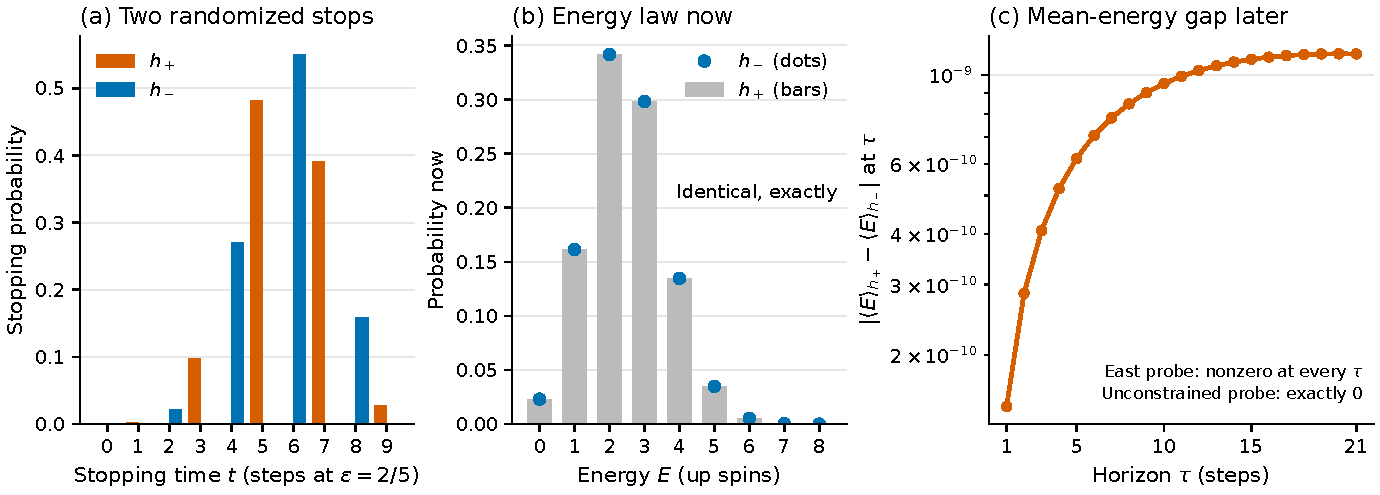
\includegraphics[width=\linewidth]{figures/out/fig_gt6_energy_witness.pdf}
  \caption{The GT6 full-energy-law witness (East $N=8$; exact rationals, floats only for
    plotting). (a) Stopping-time distributions of the two preparations, read off the positive and
    negative parts of one null vector of the current energy distributions. (b) Their current
    energy distributions coincide exactly. (c) Their future mean energies differ at every horizon
    from $1$ to $21$; the gaps are small but exactly nonzero. With the probe kernel replaced by the
    unconstrained heat bath, every gap is exactly zero.}
  \label{fig:gt6-witness}
\end{figure}

Three remarks fix how far this reaches. First, the logic is elementary. If some function $F$ mapped
the current energy law to the future, equal current laws would force equal futures, and the
certificate exhibits equal current laws with unequal futures. The exactness of the arithmetic is
what makes a $10^{-10}$ gap a proof rather than a rounding artifact. Second, the gap is tiny, and
we claim nothing about its experimental detectability. A total-variation argument gives an
explicit, equally tiny, robustness margin: perturbing each source law by at most $d/32$, with $d$
the smallest gap, keeps every future gap above $d/2$. Nonfactorization survives such a
perturbation only if the perturbed preparations still have equal current energy laws. Third, the
two preparations are independent random stopping mixtures, an explicit extension of the
deterministic-run catalog; that extension is declared, not hidden.

The ablation is the control that makes the result about the East constraint. The unconstrained
heat bath at $\epsilon=2/5$ moves the energy by one unit with probabilities that depend only on the
energy itself ($(8-j)(2/7)/8$ up and $j(5/7)/8$ down at energy $j$), so equal energy laws stay equal
forever. The separation in Fig.~\ref{fig:gt6-witness}c therefore comes from the kinetic
constraint, through the arrangement of up spins that the energy law does not record.

\subsection{The fuller filing, and why it does not pass}

The framework's complete strict-extension filing asks for more than nonfactorization. Its gate
table (Table~\ref{tab:gt6-gate-table}) includes a stability gate, G\_stab, which requires the
packaging map $E_{\tau,f}$ of \S\ref{sec:methods} to have multiple stable fixed-point strata, one
per persistent memory class.

\claimref{NEG.gt6\_original\_filing\_failed}{f90170ec0bd98b32a6c910a855ba92599bfd7ad8fa5fa930c08a04ddcb7ee82e}
On this shell that gate fails, and provably cannot be repaired by tighter numerics. At
$\epsilon=2/5$ and $\tau=1$, the packaging kernel is irreducible (an exact graph check) and
preserves the Gibbs law; a finite irreducible stochastic kernel has exactly one stationary
probability law, so there are no multiple fixed-point strata to find. Its maximum
prototype-retention error is $5/7$, far from small. That the set of reached support labels
saturates does not certify fixed points. The full filing verdict is therefore \texttt{failed},
while the object-map verdict above stands. Restoring the full filing would need a different
completion or limit construction with its own applicability proof; the finite-window persistence
of Fig.~\ref{fig:gt6-witness}c is not substituted for the missing gate. Semantic exclusions in the
admissibility domain are recorded as pending rather than assumed clear.

\begin{longtable}{lllp{6.5cm}}
\caption{GT6 gate table of the original strict-extension filing, as filed in the audit artifact}\label{tab:gt6-gate-table} \\
\toprule
gate & required & status & evidence \\
\midrule
\endfirsthead
\toprule
gate & required & status & evidence \\
\midrule
\endhead
\bottomrule
\endfoot
G\_suff & yes & pass & actual current-retaining finite maps \\
G\_desc & no & not\_required & glass bridge claims strict object-map enrichment, not closed macro dynamics \\
G\_stab & yes & failed & requires packaging fixed points; support-label saturation is insufficient \\
G\_ctrl & yes & pass & same-source unconstrained probe ablation \\
G\_nosmuggle & yes & pass & current-only convex selector \\
G\_vis & yes & pass & actual citations and scoped nonclaims \\
G\_audit & yes & pass & exact certificate source replay \\
G\_strict & yes & strict\_pass & same-shell full-energy-law split pair; F-III T12/T13 \\
G\_locglob & no & not\_required & shell-bound single bridge only; no stacked or glued promotions claimed \\
\bottomrule
\end{longtable}


The knockout panel (Table~\ref{tab:gt6-knockouts}) disables, in turn, each of the six primitives
P1--P6 that the framework says a closed description can depend on, and records the effect in two
distinct modes. For P1--P3 the knockouts are \emph{numeric}: the primitive is replaced (identity
run kernels; the unconstrained lumpable kernel; constant $\epsilon$) and a declared numeric
diagnostic degrades past its declared threshold. For P4--P6 they are \emph{capability-loss}
rows: removing the primitive makes a downstream diagnostic unavailable rather than numerically
degraded, and no numeric threshold is claimed. Two rows use auxiliary systems: P5 uses an $N=8$
packaging diagnostic, and P6 uses a separate three-state system with a two-phase clock. Because of
this, the panel is a scoped diagnostic survey. It does not show that six primitives act causally
in one glass dynamics, and no full-loop lawfulness is claimed.

\begin{longtable}{lllp{6.5cm}}
\caption{GT6 knockout panel (P1--P3 numeric ablations; P4--P6 capability-loss rows)}\label{tab:gt6-knockouts} \\
\toprule
primitive & kind & degraded & threshold \\
\midrule
\endfirsthead
\toprule
primitive & kind & degraded & threshold \\
\midrule
\endhead
\bottomrule
\endfoot
P1 & numeric & True & identity trace variation must be exactly 0 \\
P2 & numeric & True & unconstrained control must be exactly lumpable under L\_energy \\
P3 & numeric & True & constant-epsilon replacement must fail the hump detector \\
P4 & capability\_loss & True & -- \\
P5 & capability\_loss & True & -- \\
P6 & capability\_loss & True & -- \\
\bottomrule
\end{longtable}


\claimref{NEG.material\_forcing\_absent}{83603ae6bd44b85dcee00a82ab0583a20c6944efc065d0fe91d0df5b5ed3cfe5}
One more route is also closed. Paper [C]'s strict-extension theorem needs \emph{material forcing}:
the protocol catalog must contain conditioned schedules, in which the next temperature step depends
on the measured panel, as in real glass processing, and some distinctions between histories must
exist only because of them. The audited catalog has
$\texttt{material\_forcing\_count} = 0$, so that theorem is not invoked anywhere. This marks the
boundary of the [C] machinery this instantiation exercises; it is not evidence about other shells
or protocols.

\subsection{Pressure: what can and cannot be said}

The filing also carries a thermodynamic-pressure diagnostic: tilt the transition kernel by
$e^{s E}$ and measure the exponential growth rate of its powers. One might hope that conditioning
on energy fibers would lower this pressure by a positive amount, a ``conditional gap''. The
exact analysis settles which versions of that hope survive.

\claimref{FINDING.gt6\_pressure\_limits}{03ce6a60bbdd32dd6f1948f86e7085788ee1b86006370ffaf332f44d71ca3cf2}
For the tilted East operator on the shell ($N=8$, $\epsilon=2/5$, tilt $s=1/5$), positive
comparison vectors and exact exponential and logarithm enclosures bound the limiting (Fekete)
pressure to $[1.039322,\, 1.039618]$. Because some power of the tilted kernel is strictly
positive, \emph{every} nonzero initial law has this same limiting pressure. Conditioning only the
initial law on an energy fiber, and then running the original dynamics, therefore gives an
infinite-time weighted gap of exactly zero. Two positive statements remain, each with its own
meaning. With the original dynamics, the finite-time Jensen contrast is certified to be at least
$1/1000$ for every horizon $n = 1, \ldots, 8$; but it is already present for the stationary
comparison law, so it is not a glass-specific witness. And killing paths when they leave an energy
fiber gives a survival-pressure contrast certified above $1/2$ ($\approx 0.6795$); killing changes
the dynamics and is not initial-law conditioning. Grade: theorem (audited class) for the stated
operator. The finite pressure ladder in the filing's support table is a float diagnostic, not a
limiting pressure.

\subsection{What strictness does not mean}

The nonclaims (Appendix~\ref{app:nonclaims}) are part of the result. Strictness here is
shell-local and finite-window: no shell-general strict-bridge theorem, no all-time persistence,
no large-$N$ statement. It does not imply that the memory layer has an autonomous closed dynamics
of its own, nor that anything drives it (no P6\_drive audit was performed). The pressure
quantities are neither closure deficits nor the strictness witness; the energy-law split pair is.
And the promotion is a single bridge $T_0 \to T_1$; the framework has no theorem for stacking
such bridges, and none is used.
